        \clearpage
        \begin{figure*}[ht]
            \pdfbookmark[2]{ID 01}{figure_id_01}
        	\centering
            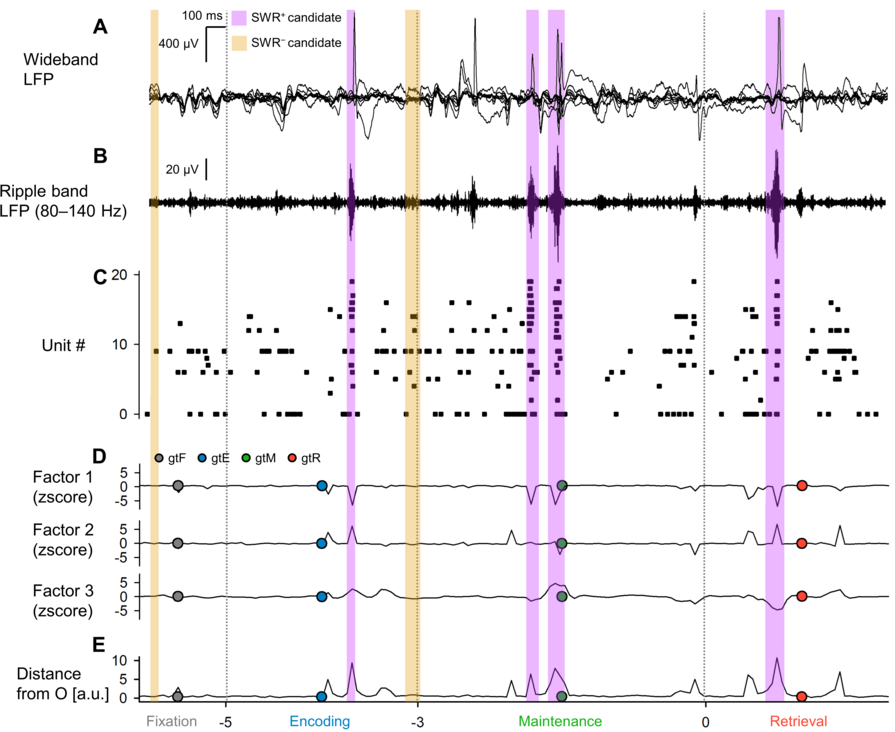
\includegraphics[width=1\textwidth]{./src/figures/.png/Figure_ID_01.png}
        	\caption{\textbf{
Local Field Potentials (LFP), Multiunit Activity, and Neural Trajectories in the Hippocampus During a Modified Sternberg Task
}
\smallskip
\\
\textbf{\textit{A.}} The presented traces illustrate representative wideband LFP intracranial EEG (iEEG) signals, recorded from the left hippocampal head while the subject was performing a modified Sternberg working memory task. This included phases of fixation (1 s, \textit{gray}), encoding (2 s, \textit{blue}), maintenance (3 s, \textit{green}), and retrieval (2 s, \textit{red}). \textbf{\textit{B.}} Subsequently, the corresponding ripple band LFP traces are delineated. \textbf{\textit{C.}} The raster plot represents multiunit spikes drawn from the LFP traces, sorted by a reliable spike-sorting algorithm \cite{niediek_reliable_2016}. \textbf{\textit{D.}} Following that, we portray the neural trajectories, which have been computed using GPFA on spike counts per unit within 50-ms bins. Each phase's geometric median is denoted by dot circles. \textbf{\textit{E.}} The distance of the trajectory from the origin $O$ is presented, with \textit{purple} and \textit{yellow} rectangles indicating the timings for SWR$^+$ candidates and SWR$^-$ candidates (acting as controls for SWR$^+$), respectively.
}
% width=1\textwidth
        	\label{fig:01}
        \end{figure*}
